% =============================================================================
% The CGAL Developers' Manual
% Chapter: Introduction
% -----------------------------------------------------------------------------
% file   : intro.tex
% authors: Susan Hert <hert@mpi-sb.mpg.de> & 
%          Stefan Schirra <stschirr@mpi-sb.mpg.de>
% -----------------------------------------------------------------------------
% $Id$
% $Date$
% =============================================================================

\chapter{Introduction\label{chap:intro}}
\ccChapterRelease{Chapter Version: 1.0}
\ccChapterAuthor{Susan Hert ({\tt hert@mpi-sb.mpg.de})\\
Stefan Schirra ({\tt stschirr@mpi-sb.mpg.de})
}

\begin{ccTexOnly}
\begin{center}
  \includegraphics[width=240pt]{Developers_manual/fig/cgal}
\end{center}
\end{ccTexOnly}

\begin{ccHtmlOnly}
<CENTER>
<IMG BORDER=0 SRC="fig/cgal_small.gif" 
  ALIGN=middle ALT="Computational Geometry Algorithms Library"><BR>
</CENTER>
\end{ccHtmlOnly}
\centerline{{\sc Computational Geometry Algorithms Library}}


\begin{quote}
{\em The goal of \cgal\ is to make available to users in industry and academia
the most important efficient solutions to basic geometric problems
developed in the area of computational geometry in a \CC\ software library.}
\end{quote}

Work on \cgal\ has been supported by {\sc esprit iv} projects 21957 (CGAL) and
28155 (GALIA).


\InternalOnly{
\section{Manual organization\label{sec:manual_org}}

This manual is meant to be a resource for developers who wish to contribute
to the \cgal\ library either by designing new packages or maintaining
or enhancing existing ones. The manual is organized roughly in the order in
which a developer will need the information in order to produce a package
for the library. We begin in this chapter with a description
of the design goals of \cgal\ and the overall design, which should be kept
in mind during all stages of development.  The remaining chapters describe
in more concrete terms the requirements and recommendations for documentation,
code writing, and testing that are derived from these goals.  We also describe
a number of tools that have been created to help in the development process
and give pointers to other sources of information.

A description of how the specification
for a package should be documented is provided along with information about
the tools available to help produce the documentation
in Chapter~\ref{chap:specification}.
Chapter~\ref{chap:svn} discusses the SVN server on which all \cgal\ source
code is kept.
Chapter~\ref{chap:directory_structure} describes the directory structure
required for a package and Chapter~\ref{chap:tools} describes a set of tools
that may be used to create or modify various files required within this
directory structure. Chapters~\ref{chap:code_format}
through~\ref{chap:robustness}
discuss issues related to the writing of code that is in keeping with
the goals of \cgal.  Chapter~\ref{chap:portability} describes issues
related to the configuration of \cgal\ and
discusses portability issues for various platforms. Chapter~\ref{chap:testing}
describes the requirements and behaviour of the test suite for a package and
Chapter~\ref{chap:debugging} consists of various hints for debugging.
Guidelines for the development of example and demo programs are given in
Chapter~\ref{chap:examples_and_demos}. Information
about how to submit a package's specification to the editorial board
for approval and the implementation (and documentation) for inclusion in
internal releases is presented in  Chapter~\ref{chap:submission}.
Chapter~\ref{chap:releases} gives information about the creation of the
internal, public, and bug-fix releases.  Chapter~\ref{chap:web_site}
provides information about the \cgal\ web site and what developers should
do to assure that it is kept up to date.
Chapters~\ref{chap:addresses} and Chapter~\ref{chap:info}
provide information about mailing lists and other information
resources developers might find useful.

}

% =============================================================================
% The CGAL Developers' Manual
% Chapter: Introduction
% -----------------------------------------------------------------------------
% file   : philosophy.tex
% authors: Stefan Schirra <stschirr@mpi-sb.mpg.de>
% -----------------------------------------------------------------------------
% $Id$
% $Date$
% =============================================================================

\section{Primary design goals\label{sec:design_goals}}
\ccIndexSubitemBegin{design}{goals}
The primary design goals of \cgal\ are \cite{fgkss-dccga-00}:

\subsection*{Correctness}
\ccIndexMainItem{correctness}
A library component is correct if it behaves according to its
specification. 
Basically, correctness is therefore a matter of 
verification that documentation and implementation coincide.
In a modularized program the correctness of a module is determined 
by its own correctness and the correctness of all the modules it depends on.  
Clearly, in order to get correct results, correct algorithms and data 
structures must be used. 

\ccIndexSubitem{correctness}{vs. exactness}
\ccIndexMainItem{exactness}
Exactness should not be confused with correctness in the sense of
reliability. There is nothing wrong with algorithms computing approximate 
solutions instead of exact solutions, as long as their 
behavior is clearly documented and they do behave as specified.
Also, an algorithm handling only non-degenerate cases can be
correct with respect to its specification, although in \cgal\ we would
like to provide algorithms handling degeneracies.\ccIndexMainItem{degeneracies} 

\subsection*{Robustness}
\ccIndexMainItem{robustness}
A design goal particularly relevant for the implementation of
geometric algorithms is robustness.  Many implementations of geometric
algorithms lack robustness because of precision problems; see 
Chapter~\ref{chap:robustness} for a discussion of robustness issues within 
\cgal.

\subsection*{Flexibility}
\ccIndexMainItem{flexibility}
The different needs of the potential application areas demand 
flexibility in the library. Four sub-issues of flexibility can be identified.

{\bf Modularity.}
\ccIndexMainItem{modularity}
A clear structuring of \cgal\ into modules with as few dependencies as
possible helps a user in learning and using \cgal, since the overall
structure can be grasped more easily and the focus can be narrowed to
those modules that are actually of interest. 

{\bf Adaptability.}
\ccIndexMainItem{adaptability}
\cgal\ might be used in an already established environment with
geometric classes and algorithms in which case the modules will 
most probably need adaptation before they can be used. 

{\bf Extensibility.}
\ccIndexMainItem{extensibility}
Not all wishes can be fulfilled with \cgal. Users may want to
extend the library. It should be possible, and in fact desirable, to
integrate new classes and algorithms into \cgal.

{\bf Openness.}
\ccIndexMainItem{openness}
\cgal\ should be open to coexist with other libraries, or better, to
work together with other libraries and programs. The \CC\ 
Standard~\cite{cgal:ansi-is14882-98}
\index{C++ standard@\CC\ standard}
\ccIndexMainItem{\stl}
defines with the \CC\ Standard Library a common
foundation for all \CC\ platforms. 
So it is easy and natural to gain openness by following this standard.
There are important libraries outside the standard, and \cgal\
should be easily adaptable to them as well.

\subsection*{Ease of Use}
\ccIndexMainItem{ease of use}
Many different qualities can contribute to the ease of use of a
library. Which qualities are most important differs according to 
the experience of the user.
The above-mentioned correctness and robustness issues are among
these qualities. Of general importance is the length of time required
before the library becomes useful. Another issue is the number of 
new concepts and
exceptions to general rules that must be learned and remembered.

Ease of use tends to conflict with flexibility, but in many
situations a solution can be found.
The flexibility of \cgal\ should not distract a novice who takes the 
first steps with \cgal.
\ccIndexSubitem{ease of use}{vs. flexibility}
\ccIndexSubitem{flexibility}{vs. ease of use}

{\bf Uniformity.}
\ccIndexMainItem{uniformity}
A uniform look and feel of the design in \cgal\ will help in learning
and memorizing. A concept once learned should be applicable in all
places where one would wish to apply it. 
A function name once learned for a specific
class should not be named differently for another class. 

\index{C++ standard@\CC\ standard} \ccIndexMainItem{\stl} \cgal\ is
based in many places on concepts borrowed from \stl\ (Standard
Template Library) or the other parts of the \CC\ Standard Library. An
example is the use of streams and stream operators in \cgal. Another
example is the use of container classes and algorithms from the
\stl. So these concepts should be used uniformly.

\index{boost} \ccIndexMainItem{boost} During the past few years,
\cgal\ has moved towards using on concepts and ideas from the boost
libraries, as well as providing interfaces towards boost
libraries. These include the boost graph libary and the boost property
maps library.

{\bf Complete and Minimal Interfaces.}
\ccIndexMainItem{completeness}
\ccIndexSubitem{interfaces}{designing}
A goal with similar implications as uniformity is a design
with complete and minimal interfaces, see for example Item 18 
in Ref.~\cite{cgal:m-ec-97}.
An object or module should be complete in its 
functionality, but should
not provide additional decorating functionality. Even if a certain
function might look like it contributes to the ease of use for a certain 
class, in a more global picture it might hinder the understanding of 
similarities and differences among classes, and make it harder to learn 
and memorize.

{\bf Rich and Complete Functionality.}
\ccIndexMainItem{completeness}
\ccIndexMainItem{functionality}
We aim for a useful and rich collection of geometric classes, data
structures and algorithms. \cgal\ is supposed to be a foundation for
algorithmic research in computational geometry and therefore needs a
certain breadth and depth. The standard techniques in the field are
supposed to appear in \cgal. 

Completeness is also related to robustness.
\ccIndexMainItem{completeness}
\ccIndexMainItem{robustness}
We aim for general-purpose
solutions that are, for example, not restricted by assumptions on
general positions. Algorithms in \cgal\ should be able to handle
special cases and degeneracies. 
\ccIndexMainItem{general position}
\ccIndexMainItem{degeneracies}
In those cases where handling of degeneracies turns out to be
inefficient, special variants that are more efficient but less general
should be provided in the library in addition to the general 
algorithms handling all degeneracies. Of course, it needs to be
clearly documented which degeneracies are handled and which are not.

\subsection*{Efficiency}
\ccIndexMainItem{efficiency}
For most geometric algorithms theoretical results for the time and space
complexity are known. Also, the theoretic interest in efficiency for
realistic inputs, as opposed to worst-case situations, is
growing~\cite{v-ffrim-97}.
For practical purposes, insight into the constant factors hidden in the
$O$-notation is necessary, especially if there are several competing
algorithms.
\ccModifierCrossRefOff
\ccIndexMainItem{implementations, multiple}
\ccModifierCrossRefOn
Therefore, different implementations should be supplied if there is 
not one best solution, as, for example, when there is a tradeoff between 
time and space or a more efficient implementation when there are no or few 
degeneracies. 
\ccIndexMainItem{time-space tradeoff}
\ccIndexSubitemEnd{design}{goals}


% =============================================================================
% The CGAL Developers' Manual
% Chapter: Introduction
% -----------------------------------------------------------------------------
% file   : overall_design.tex
% authors: Stefan Schirra <stschirr@mpi-sb.mpg.de>
% -----------------------------------------------------------------------------
% $Id$
% $Date$
% =============================================================================

\section{The overall design\label{sec:overall_design}}
\ccIndexMainItem{design}

The design goals, especially flexibility and efficient robust 
computation, have led us to opt for the generic programming paradigm using 
templates in \CC.\footnote{In appropriate places, however, \cgal\ does 
and should make use of object-oriented solutions and design patterns, as well.}
In the overall design of \cgal\ two major layers can be identified, the
layer of algorithms and data structures and the kernel layer
(Figure~\ref{fig:genericCGAL}).
\ccIndexMainItem{kernel}

\begin{figure}
\begin{ccTexOnly}
\begin{center}
  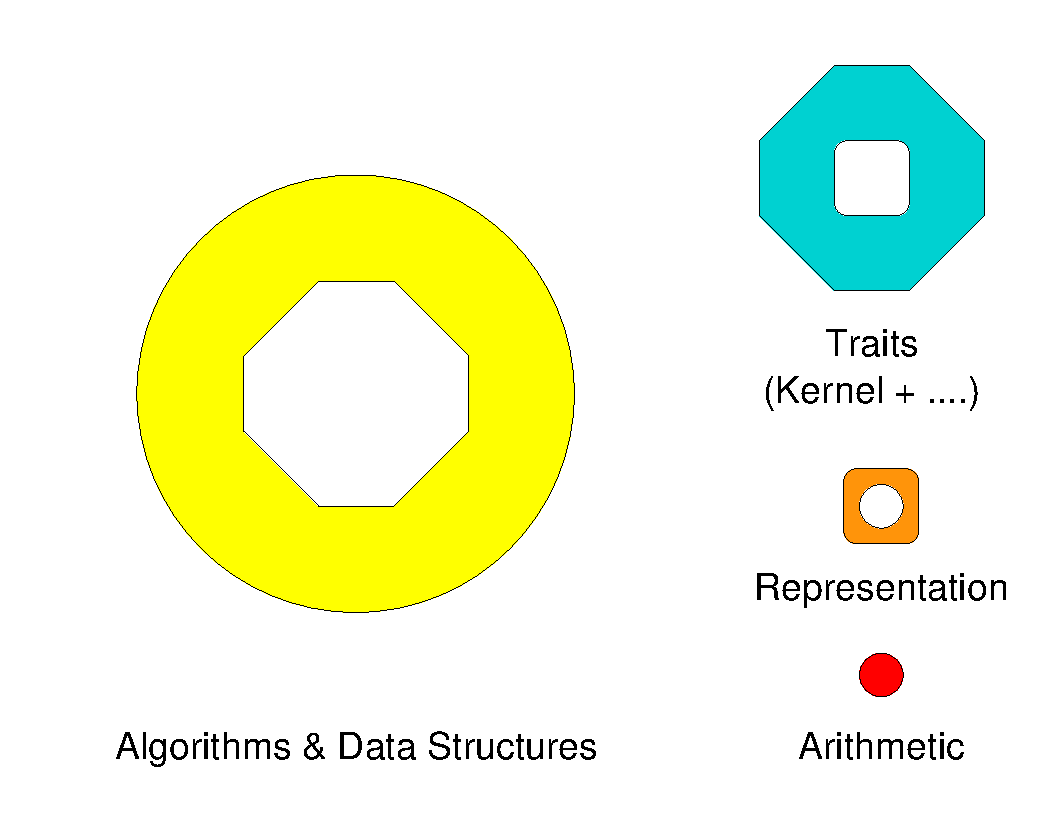
\includegraphics[width=10cm]{Developers_manual/fig/generic_cgal}
\end{center}
\end{ccTexOnly}
\caption{The generic design of \cgal.
\label{fig:genericCGAL}}

\begin{ccHtmlOnly}
<CENTER>
<IMG BORDER=0 SRC="fig/generic_cgal.gif" 
  ALIGN=middle ALT="Generic design of CGAL">
</CENTER>
\end{ccHtmlOnly}
\end{figure}

Algorithms and data structures in \cgal\ are parameterized by the 
types of objects and operations they use. They work with any concrete 
template arguments that fulfill certain syntactical as well as semantic
requirements. In order to avoid long parameter lists,
the parameter types are collected into a single class, called the
traits class in \cgal\ccIndexMainItem{traits class}
(Chapter \ref{chap:traits_classes}.)
A {\em concept}\ccIndexMainItemDef{concepts} is an abstraction of a type 
defined by a set of requirements.
Any concrete type is called a {\em model}\ccIndexMainItemDef{model} for a 
concept if it fulfills
the set of requirements corresponding to the concept. Using this terminology,
we can say a \cgal\ algorithm or data structure comes with a traits 
concept and can be used with any concrete traits model for this concept.
Further contributions to \cgal\ should continue the current high
level of genericity. 

\cgal\ defines the concept of a geometry kernel.%
\ccIndexSubitem{kernel}{concept}
Ideally, any
model for this concept can be used with any \cgal\ algorithm. This holds, 
of course, only if the requirements of an algorithm or data structure on its
traits class are subsumed by the kernel concepts, {\em i.e.}, if an
algorithm or data structure has no special requirements 
not covered in the definition of the kernel concept. 

\cgal\ currently provides four models for the \cgal\ 2D and 3D kernel
concept. Those are again parameterized and differ in their 
representation of the geometric objects and the exchangeability of
the types involved. 
In all cases the kernels are parameterized by a number type, which
is used to store coordinates and which determines the basic arithmetic
of the kernel primitives.  See Chapter~\ref{chap:kernels} for more details.

There are further complementary layers in \cgal. The most basic layer is 
the configuration layer.\ccIndexMainItem{configuration layer}
This layer takes care of setting configuration flags according to the outcome
of tests run during installation.  The {\em support library} layer
\ccIndexMainItemDef{support library} is documented in
the \ccAnchor{http://www.cgal.org/Manual/doc_html/frameset/fsSupport.html}{Support Library Reference Manual} and contains packages
that deal with things such as visualization, number types, streams, and
\stl\ extensions in \cgal.





